\documentclass{article}\usepackage[]{graphicx}\usepackage[]{xcolor}
% maxwidth is the original width if it is less than linewidth
% otherwise use linewidth (to make sure the graphics do not exceed the margin)
\makeatletter
\def\maxwidth{ %
  \ifdim\Gin@nat@width>\linewidth
    \linewidth
  \else
    \Gin@nat@width
  \fi
}
\makeatother

\definecolor{fgcolor}{rgb}{0.345, 0.345, 0.345}
\newcommand{\hlnum}[1]{\textcolor[rgb]{0.686,0.059,0.569}{#1}}%
\newcommand{\hlsng}[1]{\textcolor[rgb]{0.192,0.494,0.8}{#1}}%
\newcommand{\hlcom}[1]{\textcolor[rgb]{0.678,0.584,0.686}{\textit{#1}}}%
\newcommand{\hlopt}[1]{\textcolor[rgb]{0,0,0}{#1}}%
\newcommand{\hldef}[1]{\textcolor[rgb]{0.345,0.345,0.345}{#1}}%
\newcommand{\hlkwa}[1]{\textcolor[rgb]{0.161,0.373,0.58}{\textbf{#1}}}%
\newcommand{\hlkwb}[1]{\textcolor[rgb]{0.69,0.353,0.396}{#1}}%
\newcommand{\hlkwc}[1]{\textcolor[rgb]{0.333,0.667,0.333}{#1}}%
\newcommand{\hlkwd}[1]{\textcolor[rgb]{0.737,0.353,0.396}{\textbf{#1}}}%
\let\hlipl\hlkwb

\usepackage{framed}
\makeatletter
\newenvironment{kframe}{%
 \def\at@end@of@kframe{}%
 \ifinner\ifhmode%
  \def\at@end@of@kframe{\end{minipage}}%
  \begin{minipage}{\columnwidth}%
 \fi\fi%
 \def\FrameCommand##1{\hskip\@totalleftmargin \hskip-\fboxsep
 \colorbox{shadecolor}{##1}\hskip-\fboxsep
     % There is no \\@totalrightmargin, so:
     \hskip-\linewidth \hskip-\@totalleftmargin \hskip\columnwidth}%
 \MakeFramed {\advance\hsize-\width
   \@totalleftmargin\z@ \linewidth\hsize
   \@setminipage}}%
 {\par\unskip\endMakeFramed%
 \at@end@of@kframe}
\makeatother

\definecolor{shadecolor}{rgb}{.97, .97, .97}
\definecolor{messagecolor}{rgb}{0, 0, 0}
\definecolor{warningcolor}{rgb}{1, 0, 1}
\definecolor{errorcolor}{rgb}{1, 0, 0}
\newenvironment{knitrout}{}{} % an empty environment to be redefined in TeX

\usepackage{alltt}
\usepackage{hyperref}
\usepackage[margin=1in]{geometry}
\usepackage{booktabs}
\IfFileExists{upquote.sty}{\usepackage{upquote}}{}
\begin{document}
% \SweaveOpts{concordance=TRUE}

\title{Manuscript outline}
\author{Christophe Rouleau-Desrochers}
\date{\today}
\maketitle

% Set Wildchrokie species shortcut
\newcommand{\Ainc}{\textit{A. incana}}
\newcommand{\Ball}{\textit{B. alleghaniensis}}
\newcommand{\Bpap}{\textit{B. papyrifera}}
\newcommand{\Bpop}{\textit{B. populifolia}}

% Set CoringTreespotters species shortcut
\newcommand{\Arub}{\textit{A. rubrum}}
\newcommand{\Asac}{\textit{A. saccharum}}
\newcommand{\Afla}{\textit{A. flava}}
\newcommand{\Bnig}{\textit{B. nigra}}
\newcommand{\Cgla}{\textit{C. glabra}}
\newcommand{\Cova}{\textit{C. ovata}}
\newcommand{\Pdel}{\textit{P. deltoides}}
\newcommand{\Qalb}{\textit{Q. alba}}
\newcommand{\Qrub}{\textit{Q. rubra}}
\newcommand{\Tame}{\textit{T. americana}}   

% 
% \begin{figure}[h!]
% 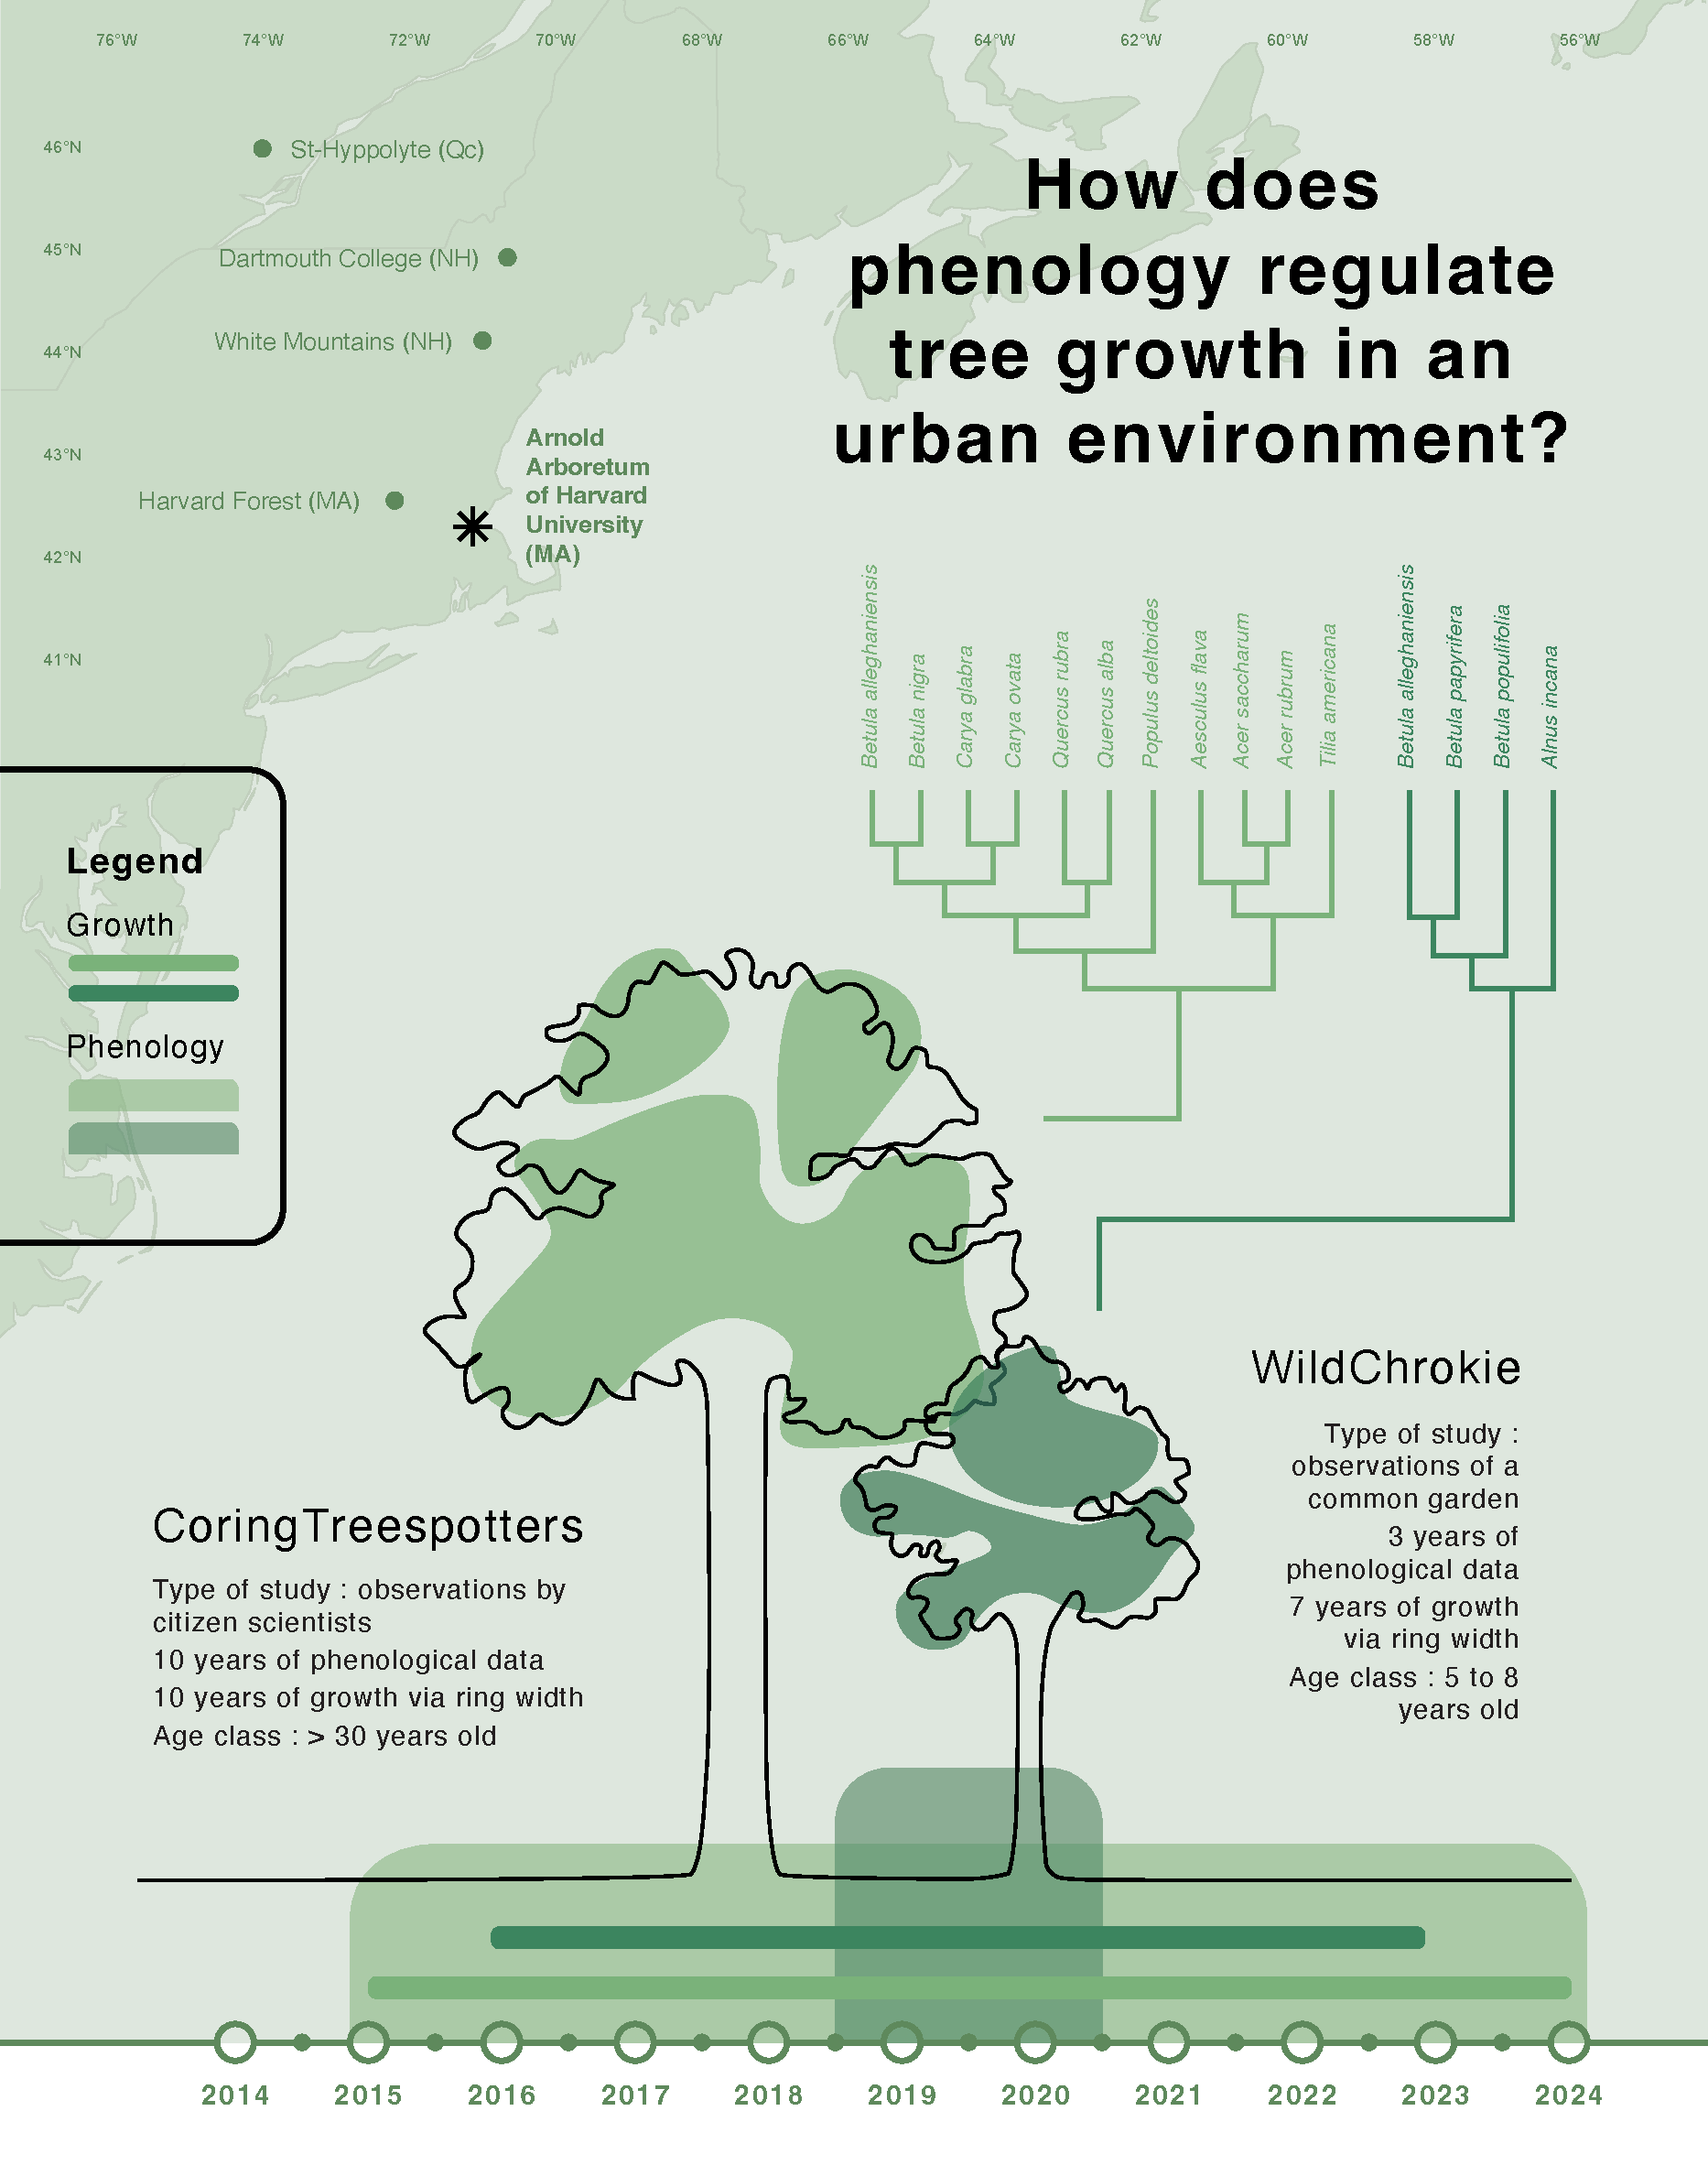
\includegraphics[width=0.85\textwidth]{../../notes/chaptersDesign/chaptersDesign.pdf}
% \caption{Overview of the age class, species, provenance of the trees used in each study along with the type of study each project consists of. The colored lines represent the period of the growth data and the shaded areas are the phenological data. Both are colour-coded by project. Each phylogram illustrates the species used in each project. The map illustrates the four different provenances used in Wildchrokie, and the star represents the location of Wildchrokie and CoringTreespotters.}
% \label{fig:chaptersDesign}
% \end{figure}

% ===========================================================================================================
\section*{Introduction}
% ===========================================================================================================
\begin{enumerate}

% Paragraph 1
\item The most frequently observed biological impact of climate change is major changes in phenology
  \begin{enumerate}
  \item Shifts in spring and autumn phenology modifies when seasons starts and ends
  \item Understanding the consequences of these shifts requires understanding how much and why growing seasons have changed 
  \item Spring phenology trends and drivers 
  \item Autumn phenology trends and drivers; shifts are weaker than springs'
  \end{enumerate}
  
% Paragraph 2
\item Shifts in spring and autumn phenology supports the assumption that longer growing seasons increase tree growth
  \begin{enumerate}
  \item Recent research shows that this may not be the case
  \item This has possible consequences on forest carbon cycle projections
  \item The different effects that shifting spring and fall events have on growth could impact these projections
  \end{enumerate}
  
% Paragraph 3
\item 
  \begin{enumerate}
  \item Understanding these finds requires answering why trees do not grow more despite longer growing seasons.
  \item We don't understand how carbon allocation to above-ground biomass, despite it being one of the largest carbon sink
  \item Trees may be source or sink limited, which enphasizes the importance of understanding the temperature sensitivity relationship between growth and photosynthesis
  \item Growth may be more sensitive to varying environmental conditions than photosynthesis, which could mislead models. 
  \item Hard nature of climate change makes uunderstanding the internal physiological constraints and external constraints to growth critical
  \end{enumerate}

% Paragraph 4
\item Growth drivers differences across species need to be considered
  \begin{enumerate} 
  \item Phenology and the relationship between growth and growing season length varies heavily accross species
  \item Polling all species together in carbon sequestrations models is a weakness
  \item We propose to use ground-based observations to address this issue
  \item These are useful to for the growth temporality of trees not suitable for experimental trials
  \item Cambial and leaf phenology are closely synchronized, so we can use them to as a proxy for start and end of season
  \end{enumerate}
  
\item How local adaptation could inform growth responses of species under future climate change

% Paragraph 5
\item Understanding the constraints to growth requires defining the growing season and growth
  \begin{enumerate}
  \item Different definitions of GS: we propose to use calendar (number of days) and thermal season (heat accumulation)
  \item Xylogenesis throughout the growing season 
  \item Tree rings as a proxy for growth
  \end{enumerate}
  
% Paragraph 6
\item Question(s?): Do trees grow more with longer growing seasons?
  \begin{enumerate}
  \item
  \end{enumerate}

\item Objectives
  \begin{enumerate}
  \item Determine if trees grow more with longer thermal vs calendar season (ref: conceptual figure)
  \item Understand the calendar growing season relationship with growth and how it relates to the SOS and EOS
  \item Determine how growth changes across species and their provenances
  \end{enumerate}
\end{enumerate}
% ===========================================================================================================
\section*{Methods}
% ===========================================================================================================
\begin{enumerate}
\item Common garden set up and location
  \begin{enumerate}
  \item Seed collection of 17 woody species across a latitudinal gradient
  \item Four sites Harvard Forest, the White mountains, Second College Grant of Dartmouth,
College, and St. Hippolyte.
  \item Seeds germinated following standard germination protocols in 2016
  \item Seedlings planted at Weld Hill
  \item Design was a randomized 16 plot blocks, with shade cloth
  \item Plots weeded and watered throughout the study, pruned in the fall of 2020
  \end{enumerate}

\item Leaf phenology observations
  \begin{enumerate}
  \item We observed leaf phenology twice per week (2018-2019) or once per week (2020)
  \item We used BBCH scale
  \end{enumerate}
  
\item Cookie collection
  \begin{enumerate}
  \item 
  \end{enumerate}
\end{enumerate}

% ===========================================================================================================
\section*{Results}
% ===========================================================================================================
Separate document

% ===========================================================================================================
\section*{Discussion}
% ===========================================================================================================
\end{document}
